\documentclass{article}

\usepackage{josuamathheader}

\begin{document}
\alglayout{1}
\def\headheight{25pt}
    \section*{Aufgabe 1}
    \begin{enumerate}[(a)]
        \item Jeder Teilring von $\C$ enthält $1$. Enthält der Teilring auch noch $\sqrt{d}$, so liegt die abelsche Untergruppe bezüglich Addition, die von $1$ und $\sqrt{d}$ erzeugt wird, auch im Teilring. Diese abelsche Gruppe ist, wie man leicht sieht, genau $\Z[\sqrt{d}]$ und liegt mit Sicherheit in jedem Teilring von $\C$, der $\sqrt{d}$ enthält. Es genügt also zu zeigen, dass $\Z[d]$ bezüglich Multiplikation abgeschlossen ist. Wegen $(a_1 + b_1\sqrt{d})\cdot (a_2 + b_2\sqrt{d}) = a_1a_2 + b_1b_2\cdot d + (b_1a_2 + a_1b_2)\cdot \sqrt{d} \in \Z[\sqrt{d}]$ folgt sofort die Behauptung.
        \item Es gilt
        \begin{align*}
            N((a + b\sqrt{-5}) \cdot (c + d\sqrt{-5})) &= N((ac - 5bd) + (bc + ad)\sqrt{-5})\\
            &= (ac - 5bd)^2 + 5 (bc + ad)^2\\
            &= a^2c^2 - 10 abcd + 25b^2d^2 + 5b^2c^2 + 10abcd + 5a^2d^2\\
            &= a^2c^2 + 5a^2d^2 + 5b^2c^2 + 25b^2d^2\\
            &= (a^2 + 5b^2)(c^2 + 5d^2)\\
            &= N(a + b\sqrt{-5}) \cdot N(c + d \sqrt{-5})
        \end{align*}
        Sei $u$ eine Einheit. Dann $\exists v$ mit $u\cdot v = 1 \implies N(u\cdot v) = 1 = N(u)\cdot N(v)$. Wegen $N(x) > 0 \forall x \in \Z[\sqrt{-5}]$ muss $N(u) = N(v) = 1$ gelten. Sei andererseits $N(u) = 1$. $u$ besitzt eine Darstellung durch $u = a + b\sqrt{-5}$. Wegen $N(u) = 1$ muss aber $b = 0$ und $a^2 = 1$ gelten. Also ist $u \in \{\pm 1\}$. Da $1$ und $-1$ offensichtlich Einheiten sind, folgt die Behauptung.
        \item $N(2) = 2^2 = 4$. Wäre $4$ reduzibel, so existierten $a, b\in \Z[\sqrt{-5}]\setminus \Z[\sqrt{-5}]^\times$ mit $a \cdot b = 2$ beziehungsweise $N(a) \cdot N(b) = N(a\cdot b) = N(2) = 4$. Wegen $a, b \notin \Z[\sqrt{-5}]^\times$ ist $N(a), N(b) > 1$. Also gilt $N(a) = N(b) = 2$. Wegen $2 < 5$ und $2\neq x^2 \forall x \in \Z$ gibt es kein $x \in \Z[\sqrt{-5}]$ mit $N(x) = 2$.
        Es gilt $2 \cdot 3 = 6 = (1 + \sqrt{-5}) \cdot (1 - \sqrt{-5})$. Daher ist die Faktorisierung von $6$ in irreduzible Elemente nicht eindeutig und $\Z[\sqrt{-5}]$ ist nicht faktoriell.
    \end{enumerate}
    \section*{Aufgabe 2}
    \begin{enumerate}[(a)]
        \item Für $x\in R\setminus \{0\}$ definieren wir die Abbildung $f_x\colon R\to R,\quad y \mapsto xy$. Es gilt $$\ker f_x = \{y\in R | xy = 0\} \overset{R \text{ nullteilerfrei}}{=} \{0\}.$$ Der Homomorphiesatz liefert uns $\operatorname{im} f_x \overset{\sim}{=}  R/\ker f_x \overset{\sim}{=} R/\{0\} \overset{\sim}{=} R$. Es existiert also ein $x' \in R$ mit $1= f_x(x') = x\cdot x'$. Damit haben wir ein Inverses für ein beliebiges $x\in R\setminus\{0\}$ gefunden. Es handelt sich bei $R$ also um einen Körper.
        \item Es gilt $x \cdot x^{n-1} = x \Leftrightarrow x\cdot (x^{n-1} - 1) = 0$. Nun setzen wir $x \neq 0$ voraus. Wegen der Nullteilerfreiheit von $R$ folgt daraus, dass $x^{n-1} = 1$ ist. Wegen $n > 1$ können wir daraus schließen, dass $x^{n-2} \cdot x = 1$. Damit haben wir für ein beliebiges Element $x\neq 0$ ein Inverses konstruiert und es muss sich bei $R$ um einen Körper handeln. \textbf{Warum ist der Körper dann endlich?}
        \item Sei $\mathfrak{p}$ ein Primideal in $R$. Dann ist $R/\mathfrak{p}$ nullteilerfrei. Sei dann $\pi$ die kanonische Projektion von $R \to R/\mathfrak{p}$. Dann gilt $\pi(x)^n = \pi(x^n) = \pi(x)$. Also ist $R/\mathfrak{p}$ ein nullteilerfreier Ring, sodass ein $n> 1$ existiert mit $x^n = x$ für alle $x\in R$. Nach Teilaufgabe $b$ ist er damit ein Körper. Das ist aber äquivalent dazu, dass $\mathfrak{p}$ ein maximales Ideal ist.
    \end{enumerate}
    \section*{Aufgabe 3}
    Da $\mathbb{F}_2$ ein Körper ist, muss $\mathbb{F}_2[X]$ euklidisch und insbesondere faktoriell sein. Daher besitzt also jedes Element eine eindeutige Zerlegung in irreduzible Elemente. Ein Element ist also genau dann irreduzibel, wenn keine solche Zerlegung mit mehr als einem Faktor $\notin \mathbb{F}_2[X]^\times$ existiert.
    Das einzige Polynom vom Grad $0$ ist $1$. Da aber $1$ eine Einheit ist, ist $1$ nicht irreduzibel. Vom Grad $n \geq 1$ gibt es im Allgemeinen $2^n$ mögliche Polynome, da es für die Koeffizienten von $1, \dots, X^{n-1}$ jeweils 2 Möglichkeiten gibt (der Koeffizient von $X^n$ muss $1$ sein, da das Polynom sonst nicht Grad $n$ hätte). Für $n = 1$ gibt es daher die beiden Möglichkeiten $X$ und $X + 1$. Da in einem Produkt von Polynomen stets der Grad addiert wird, müsste in einer Produktdarstellung von $X$ oder $X+1$ einer der beiden Faktoren Grad 1 und der andere Grad 0 besitzen. Das einzige Polynom vom Grad 0 ist aber eine Einheit. Daher sind $X$ und $X + 1$ irreduzibel. 
    Für $n = 2$ erhalten wir nach unserer Rechnung 4 Polynome. Allerdings haben alle Produkte zweier Polynome vom Grad 1 Grad 2. Daher sind die Polynome $X^2, X (X + 1) = X^2 + X$ und $(X + 1)^2 = X^2 + X + X + 1 = X^2 + 1$ reduzibel. Da sich jedes reduzible Polynom vom Grad 2 als Produkt von irreduziblen Polynomen vom Grad 1 schreiben lässt, $X^2 + X + 1$ aber nicht in der Liste aller dieser Produkte auftaucht, muss es irreduzibel sein.
    
    Für $n = 3$ erhalten wir $8$ Polynome. Polynome vom Grad 3 sind genau dann reduzibel, wenn man sie entweder als Produkt von drei irreduziblen Polynomen vom Grad 1 oder als Produkt eines irreduziblen Polynoms vom Grad 1 mit einem irreduziblen Polynom vom Grad 2 darstellen kann. Daher sind genau die 6 Polynome 
    \begin{enumerate}
        \item $X^3$
        \item $X^2(X + 1) = X^3 + X^2$
        \item $X(X+1)^2 = X(X^2 + 1) = X^3 + X$
        \item $(X + 1)^3 = (X^2 + 1)(X + 1) = X^3 + X^2 + X + 1$
        \item $X(X^2 + X + 1) = X^3 + X^2 + X$
        \item $(X + 1)(X^2 + X + 1) = X^3 + X^2 + X^2 + X + X + 1 = X^3 + 1$
    \end{enumerate}
    reduzibel und die verbleibenden 2 Polynome $X^3 + X + 1$ sowie $X^3 + X^2 + 1$ sind irreduzibel.

    Für $n = 4$ erhalten wir $16$ Polynome. Genau die Polynome, bei denen der konstante Term 0 ist, sind Vielfache von $X$. Damit können wir bereits $8$ Polynome ausschließen. Die verbleibenden irreduziblen Polynome lassen sich alle als Produkt von 
    \begin{enumerate}
        \item 4 irreduziblen Polynomen vom Grad 1 oder 
        \item 2 irreduziblen Polynomen vom Grad 1 und einem irreduziblen Polynom vom Grad 2 oder
        \item 2 irreduziblen Polynomen vom Grad 2 oder
        \item einem irreduziblen Polynom vom Grad 1 und einem irreduziblen Polynom vom Grad 3
    \end{enumerate}
    schreiben.
    Da wir bereits alle Vielfachen von $X$ ausgeschlossen haben, erhalten wir die reduziblen Polynome
    \begin{enumerate}
        \item $(X + 1)^4$
        \item $(X + )^2 \cdot (X^2 + X + 1)$
        \item $(X^2 + X + 1)^2$ und
        \item $(X + 1)\cdot (X^3 + X + 1)$ sowie $(X + 1)(X^3 + X^2 + 1)$.
    \end{enumerate}
    Damit bleiben $8 - 5 = 3$ irreduzible Polynome vom Grad 4 übrig.
    \section*{Aufgabe 4}
    \begin{enumerate}[(a)]
        \item $f \coloneqq (X -1)^3$, $g \coloneqq \frac{1}{(X-1)^2}$.
        \item Behauptung: $X^2 + 1$ ist irreduzibel in $\R[X]$. 
        \begin{proof}
            Will man $X^2 + 1$ als Produkt von zwei Nichteinheiten schreiben, so müssen beide Faktoren mindestens Grad 1 haben, da alle Elemente vom Grad 0 $\in \R$ liegen und damit Einheiten sind. Da sich beim Multiplizieren von Polynomen der Grad addiert, müssen beide Faktoren genau Grad 1 haben. Da der Leitkoeffizient 1 ist, setzen wir o.B.d.A. $X^2 + 1 = (x + a)(x + b) = x^2 + (a + b)x + ab$. Durch Koeffizientenvergleich folgt $a = -b$ und $1 = ab = (-b) \cdot b = -b^2$. Da Quadrate in $\R$ stets positiv sind, ist dies ein Widerspruch. Also ist $X^2 + 1$ irreduzibel in $\R[x]$.
        \end{proof}
        \item Behauptung: Das Ideal $(X,2)$ ist kein Hauptideal.
        \begin{proof}
            Wir nehmen an, $(X,2)$ ist ein Hauptideal, $(x, 2) = (f)$. Dann $\exists c\in \Z\colon\;2 = c\cdot f$. Betrachtet man die Grade in dieser Gleichheit, so erhält man $0 = \deg c + \deg f \implies \deg c = \deg f = 0$. Wegen $\deg f = 0$ kann aber $X$ nicht in $(f)$ liegen, Widerspruch!
        \end{proof}
        \item Für $R = \Z[X]$ ist $(X + 2)$ offensichtlich ein Primideal. Es gilt aber wegen Aufgabe $(c)$ die folgende Inklusion: $(X + 2) \subsetneq (X,2) \subsetneq \Z[X]$. Daher ist $(X + 2)$ kein maximales Ideal.
        \item $\Z[X]$ ist nach LA2 faktoriell, aber $(2) + (X) \neq \Z[x] = (1) = (\operatorname{ggT}(2, X))$.
        \item $\Z/2\Z(X_1,X_2,\dots)$ ist ein Körper mit unendlich vielen Elementen. Außerdem gilt $1 + 1 = 0$ und damit $p = 2 > 0$.
    \end{enumerate}
    \section*{Bonusaufgabe}
    \begin{enumerate}[(a)]
        \item 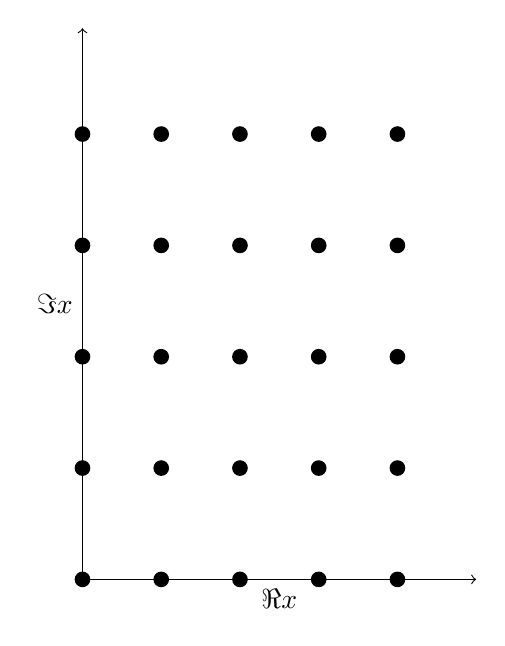
\begin{tikzpicture}
            \draw[->] (0,0) -- node[left] {$\Im x$} (0,7);
            \draw[->] (0,0) -- node[below] {$\Re x$} (5,0);
            \foreach \x in {0,1,2,3,4} \foreach \y in {0,1,2,3,4} \node[fill = black, shape = circle, inner sep=2pt] at (\x,1.414 * \y) {};
        \end{tikzpicture}
        Es gilt
        \begin{align*}
            N((a + b\sqrt{-2}) \cdot (c + d\sqrt{-2})) &= N((ac - 2bd) + (bc + ad)\sqrt{-2})\\
            &= (ac - 2bd)^2 + 2 (bc + ad)^2\\
            &= a^2c^2 - 4abcd + 4b^2d^2 + 2b^2c^2 + 4abcd + 2a^2d^2\\
            &= a^2c^2 + 2a^2d^2 + 2b^2c^2 + 4b^2d^2\\
            &= (a^2 + 2b^2)(c^2 + 2d^2)\\
            &= N(a + b\sqrt{-2}) \cdot N(c + d \sqrt{-2})
        \end{align*}, die Normfunktion ist also multiplikativ.
        
        Wir zeigen nun die Nullteilerfreiheit.
        Seien dafür $a, b, c, d\in \Z$ und $ 0 = (a + b\sqrt{-2})(c + d\sqrt{-2}) = ac -2bd + \sqrt{-2}(bc + ad)$. Koeffizientenvergleich liefert $ac = 2bd \implies abc = 2b^2d$ und $bc = -ad$. Setzen wir die zweite Gleichung in die erste ein, so ergibt sich $-a^2 d = 2b^2 d \implies -a^2 = 2b^2$. Da Quadrate stets größer 0 sind, müssen beide Seiten 0 sein, $a = b = 0$. Damit ist bereits einer der beiden Faktoren 0 und $\Z[\sqrt{-2}]$ ist nullteilerfrei.
        Sei nun $z = c + d\sqrt{-2}$. Wir zeigen, dass $\exists z' \coloneqq (a + b \sqrt{-2})\in \Z[\sqrt{-2}]$ mit $N(z - z') \leq \frac{3}{4}$. 
        
        Es gilt $N(z - (a +b\sqrt{-2})) \leq \frac{3}{\sqrt{4}} \equals (c-a)^2 + 2(d-b)^2 \leq \frac{1}{2}$. Zu jeder reellen Zahl $x$ gibt es eine ganze Zahl $n(x)$, sodass $|n(x) - x| \leq \frac{1}{2}$. Wähle also $a = n(c)$ und $b = n(d)$. Dann ist $(c-a)^2 + (d-b)^2 \leq \left(\frac{1}{2}\right)^2 + 2\left(\frac{1}{2}\right)^2 = \frac{3}{4}$.

        Seiein schließlich $z, w\in \Z[\sqrt{-2}]$ vorgegeben. Es genügt zu zeigen, dass $\exists q\in \Z[\sqrt{-2}]$ mit $N(r) = N(z - qw) < N(w)$. Wir betrachten dazu zunächst $\tilde q \coloneqq \frac{z}{w}$. Nun gibt es, wie vorhin bewiesen, zu $\tilde q$ ein $1\in \Z[\sqrt{-2}]$ mit $N(\tilde q - q) \leq \frac{3}{4}$. Nun gilt $N(z - qw) = N((\tilde q - q)w) = N(\tilde q - q) \cdot N(w) \leq \frac{3}{4} N(w) < N(w)$. Damit ist bewiesen, dass $Z[\sqrt{-2}]$ euklidisch ist.
        \item Sei $u$ eine Einheit. Dann $\exists v$ mit $u\cdot v = 1 \implies N(u\cdot v) = 1 = N(u)\cdot N(v)$. Wegen $N(x) > 0 \forall x \in \Z[\sqrt{-2}]$ muss $N(u) = N(v) = 1$ gelten. Sei andererseits $N(u) = 1$. $u$ besitzt eine Darstellung durch $u = a + b\sqrt{-2}$. Wegen $N(u) = 1$ muss aber $b = 0$ und $a^2 = 1$ gelten. Also ist $u \in \{\pm 1\}$. Da $1$ und $-1$ offensichtlich Einheiten sind, folgt die Behauptung.
        \item Es gilt $x^3 = y^2 + 2 = (y + \sqrt{-2})(y - \sqrt{-2})$. Wegen $y + \sqrt{-2} = y - \sqrt{-2} + 2\sqrt{-2}$ ist mithilfe des euklidischen Algorithmus $$N(\underbrace{\operatorname{ggT}(y + \sqrt{-2}, y - \sqrt{-2})}_{\eqqcolon b}) \leq N(2\sqrt{-2}) = 8.$$ Wäre aber $y + \sqrt{-2} = (c + d\sqrt{-2}) \cdot 2 \sqrt{-2}$, so wäre nach Koeffizientenvergleich $1 = 2c$ mit $c\in \Z$. Das ist aber ein Widerspruch. Also ist $N(b) \neq 2\sqrt{-2}$, aber $b | 2 \cdot \sqrt{-2} = -\sqrt{-2}^3$. Da $\Z[\sqrt{-2}]$ faktoriell ist, muss also $b = \pm 1$, $b = \pm \sqrt{-2}$ oder $b = \pm \sqrt{-2}^2 = \pm 2$ sein. Sei also $b = \pm \sqrt{-2}$. Dann erhalten wir $y + \sqrt{-2} = (\eta + \xi \sqrt{-2})\cdot b = \pm (\eta\sqrt{-2} -2 \xi) \implies y$ gerade. Ist $y$ gerade, so folgt $x^3 = (2d)^2 + 2 = 4d + 2$. Daher muss $x$ ebenfalls gerade sein, $x = 2c$. Betrachten wir die resultierende Gleichung $8c^3 = 4d^2 + 2$ modulo 4, so ergibt sich $0 = 2$. Das ist ein Widerspruch und $y$ muss ungerade sein.
        Sei daher $b = \pm 2$. Dann erhalten wir $y + \sqrt{-2} = (\eta + \xi \sqrt{-2})\cdot b = \pm (2\eta + 2\xi\sqrt{-2}) \implies 2\eta = 1$ mit $\eta \in \Z$. Das ist ein Widerspruch. Also bleibt nur noch $b = \pm 1$, sodass $y + \sqrt{-2}$ und $y -\sqrt{-2}$ teilerfremd sein müssen.

        Da $\Z[\sqrt{-2}]$ faktoriell ist, muss es eine eindeutige Darstellung durch irreduzible Faktoren geben. Wegen $x^3 = (y + \sqrt{-2}) \cdot (y - \sqrt{-2})$, wobei auf der rechten Seite ein Produkt von teilerfremden Faktoren steht, müssen beide Faktoren auf der rechten Seite selbst schon dritte Potenzen in $\Z[\sqrt{-2}]$ sein. Daraus ergibt sich die Gleichung
        \begin{align*}
            y + \sqrt{-2} &= (a + b\sqrt{-2})^3\\
            &= a^3 + 3a^2b\sqrt{-2} -6ab^2 -2 b^3\sqrt{-2}\\
            &= a^3 - 6ab^2 + (3a^2b - 2b^3)\sqrt{-2}
        \end{align*}
        Durch Koeffizientenvergleich erhalten wir $y = a^3 - 6ab^2$ und $1 = 3a^2b - 2b^3 = b(3a^2 - 2b^2)$. Wegen $a,b\in \Z$ folgt aus dieser zweiten Gleichung $b = \pm 1$ und damit $1 = \pm (3a^2 - 2)$. Aus $1 = 3a^2 - 2$ folgt $a = \pm 1$, aus $1 = -3a^2 + 2$ folgt $3a^2 = 1$, was ein Widerspruch ist. Also ist $a = \pm 1$ und damit $(3a^2 - 2b^2) = 1 \implies b = 1$. Daraus folgt bereits 
        \[
            y = a(a^2 - 6b^2) = \pm (1 - 6) = \pm 5.  
        \]
        Daher ist $x^3 = y^2 + 2 = 27 \implies x = 3$. Damit sind $(3,5)$ und $(3,-5)$ die einzigen Lösungen dieser Gleichung mit ganzen Zahlen $x$ und $y$. Also ist tatsächlich 26 die einzige Zahl, die auf eine Quadratzahl folgt und deren Nachfolger eine Kubikzahl ist.
    \end{enumerate}
\end{document}